%                 Doubly-Stopped Binomial Distribution
%                        Kane and Zelterman
\typeout{}\typeout{}\typeout{}\typeout{}
\typeout{ Two-Stage, Phase II Designs }
\typeout{}\typeout{}
\typeout{ Michael Kane \& Dan Zelterman }
\typeout{}\typeout{}\typeout{}\typeout{}

\documentclass[12pt]{article}         %LaTeX preamble
\parskip   .4em
\jot  2ex
\parindent .3in
\textwidth      6.5in
\oddsidemargin    0in
\textheight 8.75in
\topmargin      -.5in
\baselineskip    26pt
\renewcommand{\baselinestretch}{1.5}
\renewcommand{\arraystretch}{.75}     % vertical spacing in tables
\usepackage{graphicx}                 % Needed to import pdf files
\usepackage{adjustbox}
\usepackage{amsmath}
\usepackage{amsfonts}
\usepackage{amsthm}
\usepackage{url}
\begin{document}

\newtheorem{prop}{Proposition}


% --------------- New command definitions ----------------------

\newcounter{bibno}%            Bibliographic counter

\def\waux{1}%                  Write number for the .AUX file

\newcommand\writelabel[2]%     Write label[#1] and value[#2] to .aux file
   {%                          General command, called by \Aexer and \Texer
     \immediate\write\waux%         Write this information to the .aux file:
          {\noexpand\newlabel{#1}%  Arguments #1, #2, and the page number
             {{#2}{\thepage}}}%     Warning: the page number will be incorrect
   }%                               because I use the \immediate command

\newcommand\bibref[1]%              Reference name and my label (#1)
   {%
    \addtocounter{bibno}{1}%        Increment the counter
    \def\biblab{\thebibno}%         name is same as counter with dot
    \writelabel{#1}{\biblab}%       Write the label to .AUX file 
    \noindent\biblab.%              Write this exercise name for \item[ ]
   }%

% -------------------  global definitions  ------------------------

\newcommand{\0}{\mbox{\boldmath $0$}}         %  bold zero in math mode
\newcommand{\bbeta}{\mbox{\boldmath $\beta$}} %  bold beta in math mode
\newcommand{\bd}{\mbox{\boldmath $d$}}        %  bold d in math mode
\newcommand{\bg}{\mbox{\boldmath $\gamma$}}   %  bold gamma in math mode
\newcommand{\blam}{\mbox{\boldmath $\lambda$}}%  bold lambda in math mode
\newcommand{\bpi}{\mbox{\boldmath $\pi$}}     %  bold pi in math mode
\newcommand{\bsig}{\mbox{\boldmath $\sigma$}} %  bold sigma in math mode
\newcommand{\bth}{\mbox{\boldmath$\theta$}}   %  bold theta in math mode
\newcommand{\dt}{\widetilde{d}}               %  d tilde in math mode
\newcommand{\m}{\mbox{\boldmath $m$}}         %  bold m in math mode
\newcommand{\M}{\mbox{\boldmath $M$}}         %  bold M in math mode
\newcommand{\mi}{{$-$}}                       %  large math minus sign
\newcommand{\n}{\mbox{\boldmath $n$}}         %  bold n in math mode
\newcommand{\ndot}{n{\rm\bf .}}               %  n sub-dot
\newcommand{\Nh}{\widehat{N}}                 %  N-hat
\newcommand{\nsp}{\hspace*{-.3in}}            %  large negative space
\newcommand{\p}{\phantom{5}}                  %  space for one digit
\newcommand{\pih}{\widehat{\pi}}              %  pi-hat
\newcommand{\pmi}{\phantom{$-$}}              %  space for wide minus
\newcommand{\ps}{\phantom{$*$}}               %  space for * footnote
\newcommand{\pc}{{\scriptsize$\bullet$}}      %  plotting dot character
\newcommand{\q}{\phantom{55}}                 %  space for two digits
\newcommand{\qs}{\hspace*{.1in}}              %  wide space
\newcommand{\re}{{\rm e}}                     %  Roman e (...to the power)
\newcommand{\bt}{\mbox{\boldmath $t$}}        %  bold t in math mode
\newcommand{\bT}{\mbox{\boldmath $T$}}        %  bold T in math mode
\newcommand{\U}{\mbox{\boldmath $u$}}         %  bold u in math mode
\newcommand{\X}{\mbox{\boldmath $X$}}         %  bold X in math mode
\newcommand{\x}{\mbox{\boldmath $x$}}         %  bold x in math mode
\newcommand{\Y}{\mbox{\boldmath $Y$}}         %  bold Y in math mode
\newcommand{\y}{\mbox{\boldmath $y$}}         %  bold y in math mode
\newcommand{\z}{\mbox{\boldmath $z$}}         %  bold z in math mode

% ------------------- my hyphenation rules ---------------------

\hyphenation{general-iza-tions}
\hyphenation{distri-bution}
\hyphenation{Zel-ter-man}

% ---------------  cover page  --------------------------------

\thispagestyle{empty}
\begin{center}
\vspace*{\fill}

{\Large\bf A Stopped Negative Binomial Distribution} \\ [1ex]

\vspace*{1.25in}
\begin{tabular}{l} 
 {\bf Michael Kane${}^*$} \\
 {\bf Daniel Zelterman}  \\[.1in]

 Department of Biostatistics \\
 School of Epidemiology  \\
 \hspace*{.15in} and Public Health  \\
 Yale University       \\
 New Haven, CT  06520  \\[.2in]

\today
\end{tabular}
\end{center}

\vspace*{\fill}

\noindent${}^*$Email address for author: {\tt
michael.kane@yale.edu}.  This research was supported by grants 
	R01CA131301, R01CA157749, R01CA148996, R01CA168733 awarded by the National Cancer Institute, and support from the Yale Comprehensive Cancer Center.

% ------------------------ Abstract ----------------------------

\newpage
\thispagestyle{empty}

\section*    {\bf   Abstract}

This paper introduces a new discrete distribution suggested by curtailed sampling rules common in early-stage clinical trials. We derive the distribution of the smallest number of independent Bernoulli($p$) trials needed in order to observe either $s$ successes or $t$ failures. The closed form expression for the distribution as well as the compound distribution are derived. Properties of the distribution are shown and discussed. A case study is presented showing how the distribution can be used to monitor sequential enrollment of clinical trials with binary outcomes as well as providing post-hoc analysis of completed trials.

\bigskip

\noindent{\bf Keywords:}  discrete distribution; curtailed sampling

% ---------------------------------------------------------------

\thispagestyle{empty}
\setcounter{page}{1}

% --------------------  1. Introduction   ----------------------
\section            {Introduction and Motivation}
% --------------------------------------------------------------


In the Simon 2-stage Phase II clinical trial [\ref{Simon 1989}], a small 
number of patients are enrolled onto a therapeutic 
protocol for an initial stage. Fore each patient, we assess either success 
or failure according to a 
clinically useful criteria. Success might include tumor response to treatment
or perhaps that the response is maintained for a minimum specified duration.
In addition to failing to achieve the primary endpoint, treatment failure 
might include adverse reaction to the drug or withdrawal due to toxicity. We 
use a large number of these early successes as evidence for whether to enroll
additional patients for a second stage. A statistically small number of 
successes in Stage I would lead us to terminate the trial without entering 
Stage II.

Consider the Phase II clinical trial that investigates the efficacy of 
iniparib in patients with breast cancer gene-associated (BRCA) ovarian 
cancer [\ref{Sanofi 2013}]. In the first stage 12 patients were treated with 
iniparib (BSI-201/SAR240550). The endpoint was defined by Response Evaluation 
Criteria in Solid Tumor (RECIST). If at least two Stage I patients succeeded,
then the trial would proceed to the next stage where additional patients were 
treated. If fewer than two of the 12 Stage I patients is successful then 
the trial would terminate. 

Our goal is to know the distribution of the sample size of the design for 
planning purposes.  If all 12 patients are enrolled at once, as in the classic 
design, then the sample size is 12. However, in most clinical trials, the 
patients are enrolled sequentially, often with one patient's outcome realized 
before the next one enters the trial. In the present example, observing two 
successful patients allows us to proceed to the next stage. Similarly 11 
observed treatment failures also ends the stage. This sampling mechanism, in 
which the experiment ends as soon as any of the endpoints is reached, is 
call {\em curtailed sampling}. Under curtailed sampling the range of the 
sample size is between two and 12.

We will assume each of the patient enrollments can be modeled as independent, identically distributed Bernoulli($p$) random variables. The realization of the trial is a sequence of these random variables that stops when either a specified number of success or failures is reached. As an example, suppose in the previously described trial, two successes were reached after enrolling 10 patients (one in the third step and one at the $10^{th}$). The trial is visualized in Fig \ref{fig:kane_viz}. The vertical axis denotes the number of successful outcomes. The horizontal axis denotes the number of patients that have been enrolled. The horizontal and vertical line segments represent endpoints for the trial. 

\begin{figure}[ht]
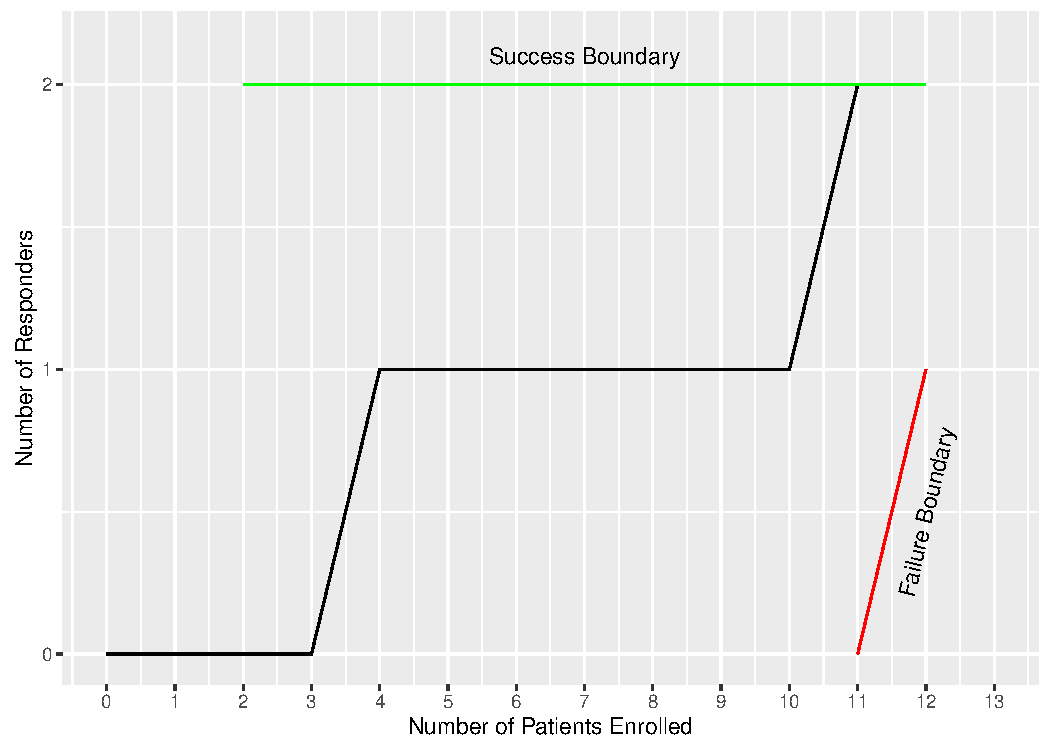
\includegraphics[width=\textwidth]{KanePlot.pdf}
\caption{
A hypothetical realization of the breast cancer trial.
}
\label{fig:kane_viz}
\end{figure}

%Our goals for this paper are three-fold. First, we derive the distribution for the number patients that need to be enrolled in the described sequential trial, which we refer to as the {\em Stopped Negative Binomial} (SNB) distribution. Using a sequential trial it is often possible to reduce the number of patients needed when compared to traditional design. Understanding of this distribution allows to create better, more {\em enrollment efficient} designs. Second, assuming a Beta distribution on the probability of success, we will derive the compound distribution of the SNB. Both the success probability and the SNB compound distribution can be updated as the individual outcome of patients are known and, as a result, better estimates of the distribution of patient-enrollment size can be derived as new data are received. Third, we will use the derived results to propose an enrollment design framework alternative to the Simon Two-stage Optimal trial design. We will show a hypothetical but representative case where the number of enrollments is less than those proposed by the Simon Two-stage and the uncertainty associated with both the individual success outcome as well as the trial is fully characterized.

The next section of this paper introduces our notation and basic results including the density of the SNB and compound SNB along with a description of it's relation to other distributions. Sections 2 and 3 derive the distribution based on a defined Bernoulli process and give some basic properties of the distribution. Section 4 derives the compound distribution using a Beta prior. Section 5 develops a post-hoc analysis of a completed trial. Section 6 is devoted to discussion and conclusions. The simulations, model fitting routines, and visualizations presented in this paper were generated using the snb package [\ref{Kane 2015}] for the R programming environment [\ref{R Core Team 2015}]

%Their individual outcomes are summarized as independent Bernoulli, %with either success according to a clinically useful criteria or else %as treatment failure. Failure might include adverse reaction to the %drug or withdrawal due to toxicity. Successes occur with probability %$\,p\; (0\leq p\leq 1)$.   

%More generally, suppose we have a sequence of independent Bernoulli$(p)\,$random variables $\,Z_1, Z_2, \ldots$. For positive integers $\,s\,$ and $\,t,$  we study the distribution of the smallest number $\,Y\,$ such that $\,Z_1, Z_2, \ldots, Z_Y\,$ %contains either $\,s\,$ successes of $\,t\,$ failures.

% ---------------------------  2. Notation ----------------------
\section   {Notation and summary of distributional results}
\label{notation.section}
% --------------------------------------------------------------

Let $\,B_1, B_2, \ldots \,$ denote a sequence of independent, identically 
distributed, Bernoulli random variables with $\mathbb{P}\{B_i=1\}=p$, for 
probability parameter $0\leq p \leq 1$. In the clinical trial setting 
$\,B_i = 0$ corresponds to a successful enrollment. 
Let $s$ and $t$ be positive integers. 
Define the stopped negative binomial (SNB) random variable $Y$ as the smallest 
integer value such that $\,\{B_1, \ldots , B_Y\}\,$ contains {\em either} 
$\,s\,$ successes or else $\,t\,$ failures. The distribution of $\,Y\,$ has 
support on integer values in the range 
\begin{equation*}                                     %   (3)
     \min(s,t) \leq \; Y \;\leq s+t-1  \label{range.y.eq}
\end{equation*}
and it is distributed as
\begin{equation} \label{eqn:pmf}
\mathbb{P}\{Y=k\} = S(k, p, s)  \{s \leq k\} + T(k, p, t) \{t \leq k \} 
\end{equation}
where
\begin{equation} \label{eqn:N}
S(k, p, s) = {k-1 \choose s-1} p^s (1-p)^{k-s} 
\end{equation}
is the negative binomial probability of $s$ successes and
\begin{equation} \label{eqn:R}
T(k, p, t) = {k-1 \choose k-t} p^{k-t} (1-p)^t
\end{equation}
is the negative binomial probability of $t$ failures.

% ------------   Section 3: Random Walk  --------------
%\section {Deriving the SNB with a Random Walk}
%\label{random.walk.section}
% --------------------------------------------------------------

To illustrate that (\ref{eqn:pmf}) is the distribution of $Y$, consider the 
process $\mathbf{X} = \{X(k) : k \in \mathbb{Z}_{\ge 0} \}$ with $X(0)=0$ and
\begin{equation*} \label{eqn:proc}
X_{k+1} = X_k + B_{k+1} \{ k-t < X_k < s \}
\end{equation*}
where $B_{k+1}$ is once again distributed as Bernoulli($p$) for all $k$ in the domain of $\mathbf{X}$. The process can be conceptualized as a series of coin flips that stops when either $s$ heads or $t$ tails are reached. At each step a coin is flipped. If it is heads, the process advances one diagonally in the positive horizontal and vertical direction. Otherwise, it advances in the positive horizontal direction only. The process stops, $X_k$'s value does not change, after either $X_k = s$ or $X_k = k-t$. One example is given in Fig. \ref{fig:kane_viz}.

\begin{prop}
The distribution of the stopping time $\{k: s \leq X_k \leq k-t \}$ is equal to the SNB and is given in (\ref{eqn:pmf}). 
\end{prop}
\begin{proof}
The proof will proceed in two parts. First, a combinatorial justification will be given for the probability mass value on each element of the support. Second, it will be shown that the sum of the masses over the support sums to one.

The probability that a given realization of $\mathbf{X}$ reaches $s$ at 
time $k$ is  the probability that, at time $k-1$ there are $s-1$ successful 
coin flips and $k-s$ unsuccessful coin flips times the probability of a 
successful coin flip at time $k$ (\ref{eqn:N}). The probability $X_k = k-t$ 
is the probability that, at time $k-1$ there are $k-t$ successful coin flips 
and $t-1$ unsuccessful coin flips times the probability of an unsuccessful 
coin flip at time $k$ (\ref{eqn:R}).  Next, we need to show that the sum
\begin{equation} \label{eqn:sum_proof}
R = \sum_{k=s}^{s+t-1} {k-1 \choose s-1} p^s (1-p)^{k-s} + \sum_{k=t}^{s+t-1} {k-1 \choose k-t} p^{k-t} (1-p)^t
\end{equation}
is equal to one.
First, substitute $i=k-s$ in the first summation and
$j=k-t$ in the second. 
\begin{equation*}
{j+s-1 \choose s-1} = {j+s-1 \choose j}
\end{equation*}
Then %(\ref{eqn:sum_proof}) becomes:
%\begin{equation*}
%R = \sum_{i=0}^{t-1} {i+s-1 \choose s-1} p^s (1-p)^i +
%\sum_{j=0}^{s-1} {j+t-1 \choose j} p^j (1-p)^t.
%\end{equation*}
$R$ can be written
as the cumulative distribution function of two 
negative binomial distributions
\begin{equation} \label{eqn:transformed_sum}
R = \sum_{i=0}^{t-1} {i+s-1 \choose i} p^s (1-p)^i \; + \;
\sum_{j=0}^{s-1} {j+t-1 \choose j} p^j (1-p)^t.
\end{equation}

Let $I_p(s, t)$ be the {\em regularized incomplete beta function}, which is 
also one minus the c.d.f. of the negative binomial distribution. This
function satisfies $I_p(s, t) = I_{1-p}(t, s)$.  Then 
\begin{align*}
R = \sum_{i=0}^{t-1} &{i+s-1 \choose i} p^s (1-p)^i +
\sum_{j=0}^{s-1}  {j+t-1 \choose j} p^j  (1-p)^t \\
   &= 1-I_p(s, t) + 1 - I_{1-p}(t, s) \\
   &= 1. 
\end{align*}
\end{proof}
Proving that \label{eqn:pmf} is a valid probability mass function.

From (\ref{eqn:pmf}) one can see that the mass at any point on the support of the distribution may come from either $X_k = s$, captured in the function $S$, or $X_k = k-t$, captured in the function $T$. The support of $S$ is defined by $s \leq S \leq s+t+1$ and the support of $T$ is defined by $t \leq T \leq s+t+1$.

\begin{figure}[p!]
\begin{center}
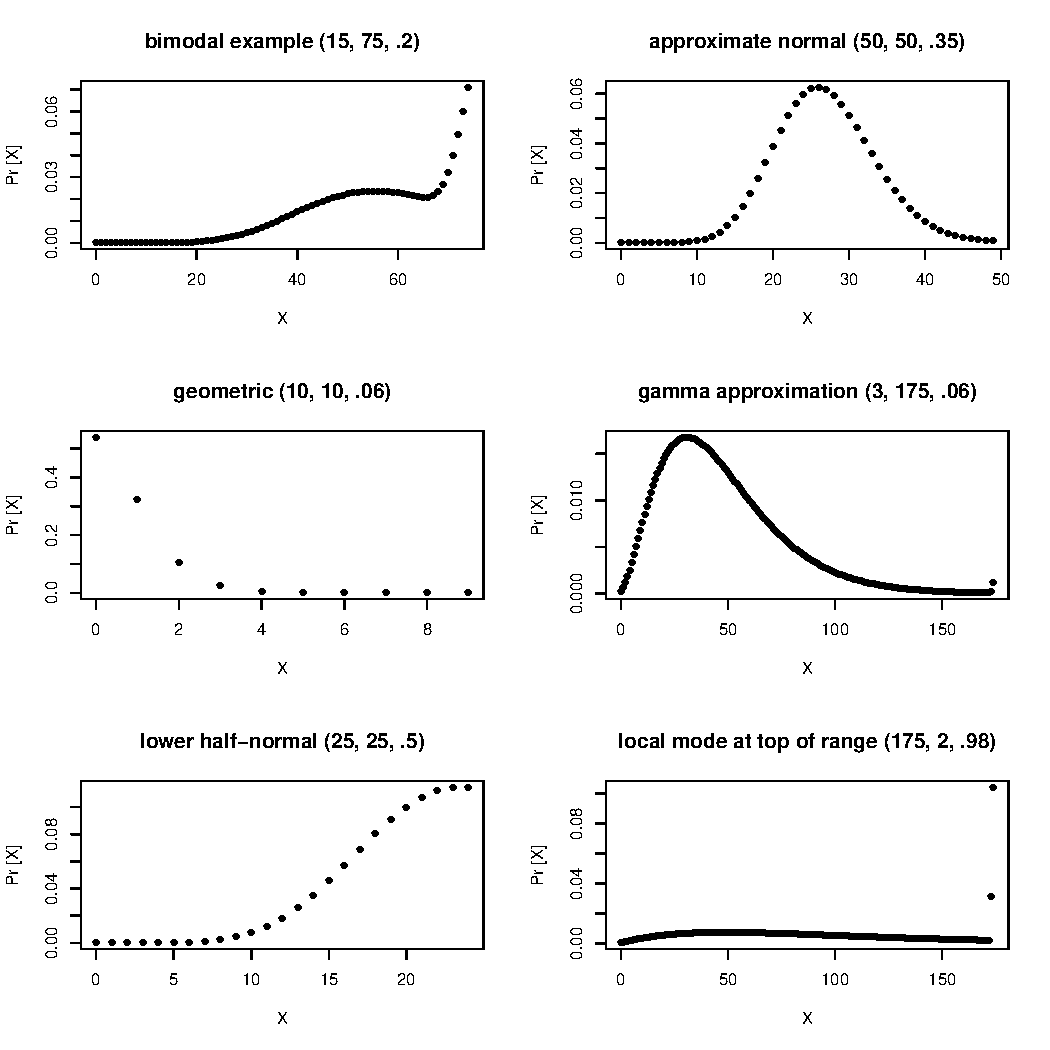
\includegraphics[scale=.9]{shapes.pdf}
\end{center}
\caption{Different shapes of the SNB distribution with parameters ($s$, $t$, $p$), as given. \label{shapes.fig}}
\end{figure}

The probability mass function of $\,Y\,$ has a variety of shapes for different choices of the parameters $(s,\, t,\,p)$.
These shapes are illustrated in Fig.~\ref{shapes.fig}.
The SNB is related to the negative binomial distribution. Specifically, if 
$t$ is infinitely large then the $Y-s$ has a negative binomial distribution 
with
\begin{equation*}                                    %   (1)
   \mathbb{P}\{Y=s+j \}        \label{nb1.eq}
          = {{s+j-1}\choose{s-1}} p^s (1-p)^j
\end{equation*}
for $\,j=0, 1,\ldots\,$. A similar statement can be made when $s$ is large
and $t$ is small.

For the special case of $\,s=t,$ the distribution of $\,Y\,$ is the riff-shuffle, or minimum negative binomial distribution~[\ref{Uppuluri 1970}].
Similar derivations of the closely-related maximum negative binomial discrete distributions also appear in~[\ref{Zhang 2000}, \ref{Zelterman 2004}].

%\subsection{Updating the SNB distribution}

%Under the presented random walk construction if the process is observed before reaching one of its endpoints the conditional distribution is a reparametrized SNB distribution whose parameters are determined by $X_k$ and $k$, the process value and time step. For example, in the breast cancer trial the distribution of the number of patients is parameterized as $SNB(2, 11, p)$. At the third enrollment there is one successful outcome. Conditioned on this information, the number of additional patient enrollments is $SNB(1, 9, p)$. As new outcomes are collected the conditional distribution can be re-derived to get better estimates of the total patient enrollment. Furthermore, if our task is to estimate $p$ along with the patient enrollment distribution, this parameter can also be updated as new data are received.  

\section{The Compound Distribution}

%The previous section derives a new distribution for a sequential Bernoulli process where the process is stopped when either a total number of successes is reached or a total number of failure is reached. The process can be alternatively conceptualize as a series of coin flips that stops when either $s$ heads or $t$ tails are reached. At each step a coin is flipped. If it is heads then one step is taken in the positive direction on the vertical axis. Otherwise, a step is taken in the positive direction on the horizontal axis. The walk stops when either $s$ is reached on the vertical axis or $t$ is reached on the horizontal axis. A visual example is shown in Fig. \ref{fig:zelterman_viz}.

%\begin{figure}[ht]
%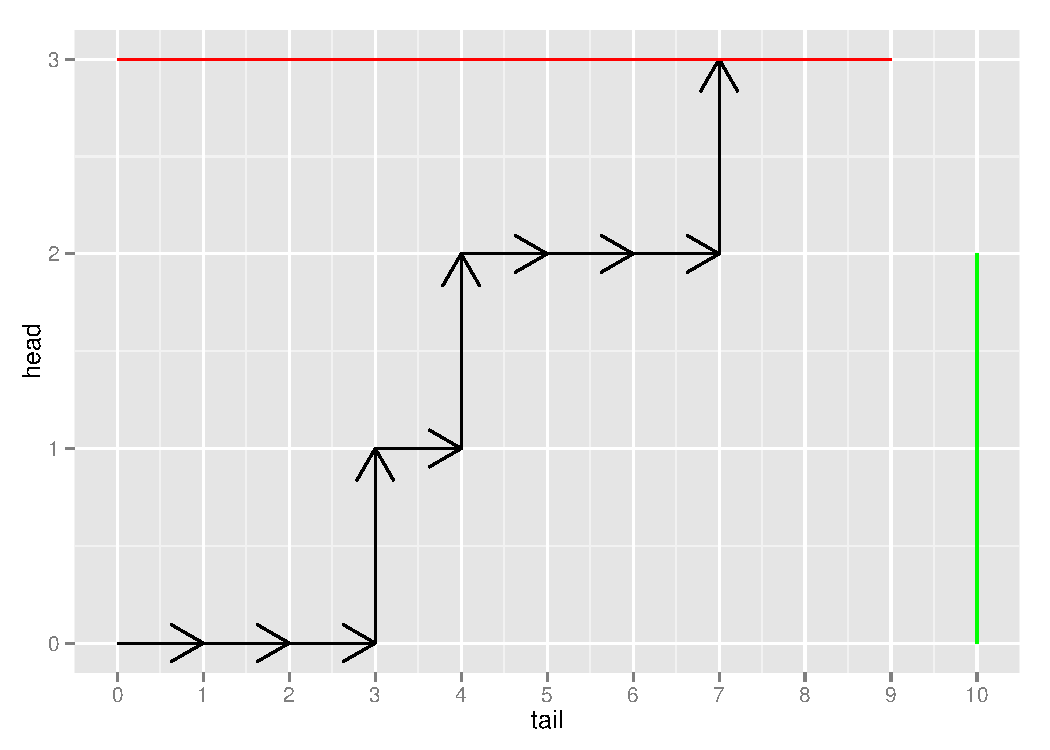
\includegraphics[width=\textwidth]{ZeltermanPlot.pdf}
%\caption{
%A realization of $\mathbb{X}$ with $p=0.3$, $s=3$, and $t=10$. An arrow to the right indicates a coin flip of ``tail'' and
%an arrow in the vertical direction indicates ``head.''
%}
%\label{fig:zelterman_viz}
%\end{figure}

If we assume that $p$ has a Beta distribution, with constant prior parameters $\alpha$ and $\beta$ then we can calculate the closed form compound distribution of the SNB as
\begin{align}
\mathbb{P} \{Y = k | \mathbf{B}, \alpha, \beta \} &= {k-1 \choose s-1} \frac{B\left(\alpha+s, k-s+\beta \right)}{B(\alpha, \beta)} \{s \leq k \leq s+k-1\} + \nonumber \\
& {k-1 \choose k-t} \frac{B\left(\alpha + k - t, t+\beta\right)}{B(\alpha, \beta)} \{t \leq k \leq s+k-1\}
\end{align}
where $B$ is the Beta function and $\mathbf{B}$ is the sequence of Bernoulli data.

When $p$ is known, the probability mass function (PMF) of the number of steps until the process is stopped is given by (\ref{eqn:pmf}). However, many times this is not the case. In Phase II clinical trials for example patients are often enrolled sequentially until there are enough patients to guarantee the desired level of power or until a specified number of adverse events are recorded. In cases such as these the endpoints $s$ and $t$ are known and we would like to be able to estimate $p$ either during enrollment to provide odds of successful enrollment or after an endpoint has been reached to determine the amount of uncertainty in the endpoint. To do this, we will assume that $p$'s probability in the absence of available data is $\text{Beta}(1/2, 1/2)$, the Jeffrey's prior. This distribution was chosen for two reasons. First, it is the conjugate prior of the (Negative) Binomial distribution and updating the distribution as data are received is straightforward. Second, it is objective and limits the number of ``prior coin-flips'' to one. This means that data are more heavily influence the distributional characteristics of $p$ with more data providing more proportional influence.

\begin{prop}
The compound PMF of the Stopped Negative Binomial distribution with a Beta($\alpha$, $\beta$) prior is:
\begin{align}
f(k | s, t, \alpha, \beta) &= {k-1 \choose s-1} \frac{B\left(\alpha+s, k-s+\beta \right)}{B(\alpha, \beta)} \{s \leq k \leq s+k-1\} + \nonumber \\
& {k-1 \choose k-t} \frac{B\left(\alpha + k - t, t+\beta\right)}{B(\alpha, \beta)} \{t \leq k \leq s+k-1\}
\end{align}
where $B$ is the Beta function.
\end{prop}
\begin{proof}
For notational simplicity, assume that $s,t \leq k \leq s+k-1$. When this is not the case appropriate terms should be removed as dictated by the indicator functions.
\begin{align*}
f(k | s, t, \alpha, \beta) = \frac{1}{B(\alpha, \beta)} & \int_0^1 {k-1 \choose s-1} p^{\alpha +s -1} \left(1-p\right)^{k-s+\beta-1} + \\
 & {k-1 \choose k-t} p^{k-t+\alpha-1}\left(1-p\right)^{t+b-1} dp \\
= \frac{1}{B(\alpha, \beta)}  {k-1 \choose s-1} & \int_0^1  p^{\alpha +s -1} \left(1-p\right)^{k-s+\beta-1} + \\
 & \frac{1}{B(\alpha, \beta)} {k-1 \choose k-t} \int_0^1  p^{k-t+\alpha-1}\left(1-p\right)^{t+b-1} dp
\end{align*}
The result follows by applying the definition of the Beta function to the integral terms.
\end{proof}

\section{A Bayesian Exploration Simon Two-stage Optimal Design}

Returning to the breast cancer trial introduced in the first section, a response rate of 2/12 in the first stage corresponds to an individual probability of responding of $p=0.1667$. The standard deviation of this probability is $\sqrt{p(1-p)/12}=0.1076$. If we were to use the Central Limit Theorem then the 95\% confidence interval around the mean would be $[-0.0442, 0.1076]$. While this approach is problematic since the number of samples (12 in this case) is small it does indicate how much uncertainty is built into the first stage. If we consider samples from both stages then the standard deviation drops to 0.0630 and the 95\% confidence interval would be $[0.0432, 0.2901]$.

These calculations expose two difficulties with the Simon Two-stage Optimal Design. First, success in the first stage is not a good indicator of success in the second stage and at the same time failure in first stage in no way implies failure in the second stage, especially when $p$ is close to it's threshold value. The variance in the estimate so large that it is a poor estimator. The second, difficulty is that the design is not {\em enrollment efficient}. That is, if the first stage is successful then additional patients are enrolled. Enrollment, especially for certain types of cancer, can be very difficult and it can taken time to find eligible patients. Furthermore, if all 12 of the patients in the first stage respond positively, should we really need to enroll additional patients?

Properly quantifying uncertainty in the process implies quantifying uncertainty in $p$, which stems from two sources. First is the number of samples we receive. Any estimate of $p$ will be based on data and generally the more data we have, the better our estimate. If the data are small, as they often are in clinical trials, the less reliable our estimate is. The second source comes from heterogeneity in the data. While models may assume that the probability of success $p$ is a single value this is often not the case in real-world data. In clinical trials for example an individuals chance of having an adverse outcome may be influenced by any number of underlying factors, which may vary across individual. In these cases $p$ may not be a single numeric value and may be better conceptualized as a realization over an entire distribution. A frequentest approach will not capture this variation.

We would like to be able to estimate $p$ and capture both sources of uncertainty. For cases where the process has not yet reached an endpoint, we would like to be able to provide updated estimates of $p$, its uncertainty, and the probabilities of hitting each endpoint. If the process has reached an endpoint, we would again like a estimate of $p$ and its uncertainty along with the probability that another endpoint could have been reached, given the data. 

\subsection{Quantifying Uncertainty in the Simon Two-stage Optimal Design}

Both of the problems in the Simon Two-stage Optimal Design stem from the fact that it fails to quantify the uncertainty in the estimate of the success probability. A framework based on Stopped Negative Binomial distribution addresses this failure and provides the added features of monitoring the trial as new results are received, providing estimates of how many new enrollees are needed to complete a trial, and quantifying the uncertainty in the success probability.

Let's start by recasting the breast cancer study in the context of the Stopped Negative Binomial framework, assuming sequential enrollment. The first stage will stop when either two positive responses are reached or 11 negative responses. This corresponds to a Stopped Negative Binomial Distribution with $s=2$ and $t=11$. Next, lets assume that, in the first stage, there were two successes. A second success could occur during the second, through a tenth enrollment. At each of these times we would like to know the estimate for $p$ along with the lower five percent quantile of the distribution.

\begin{figure}[ht]
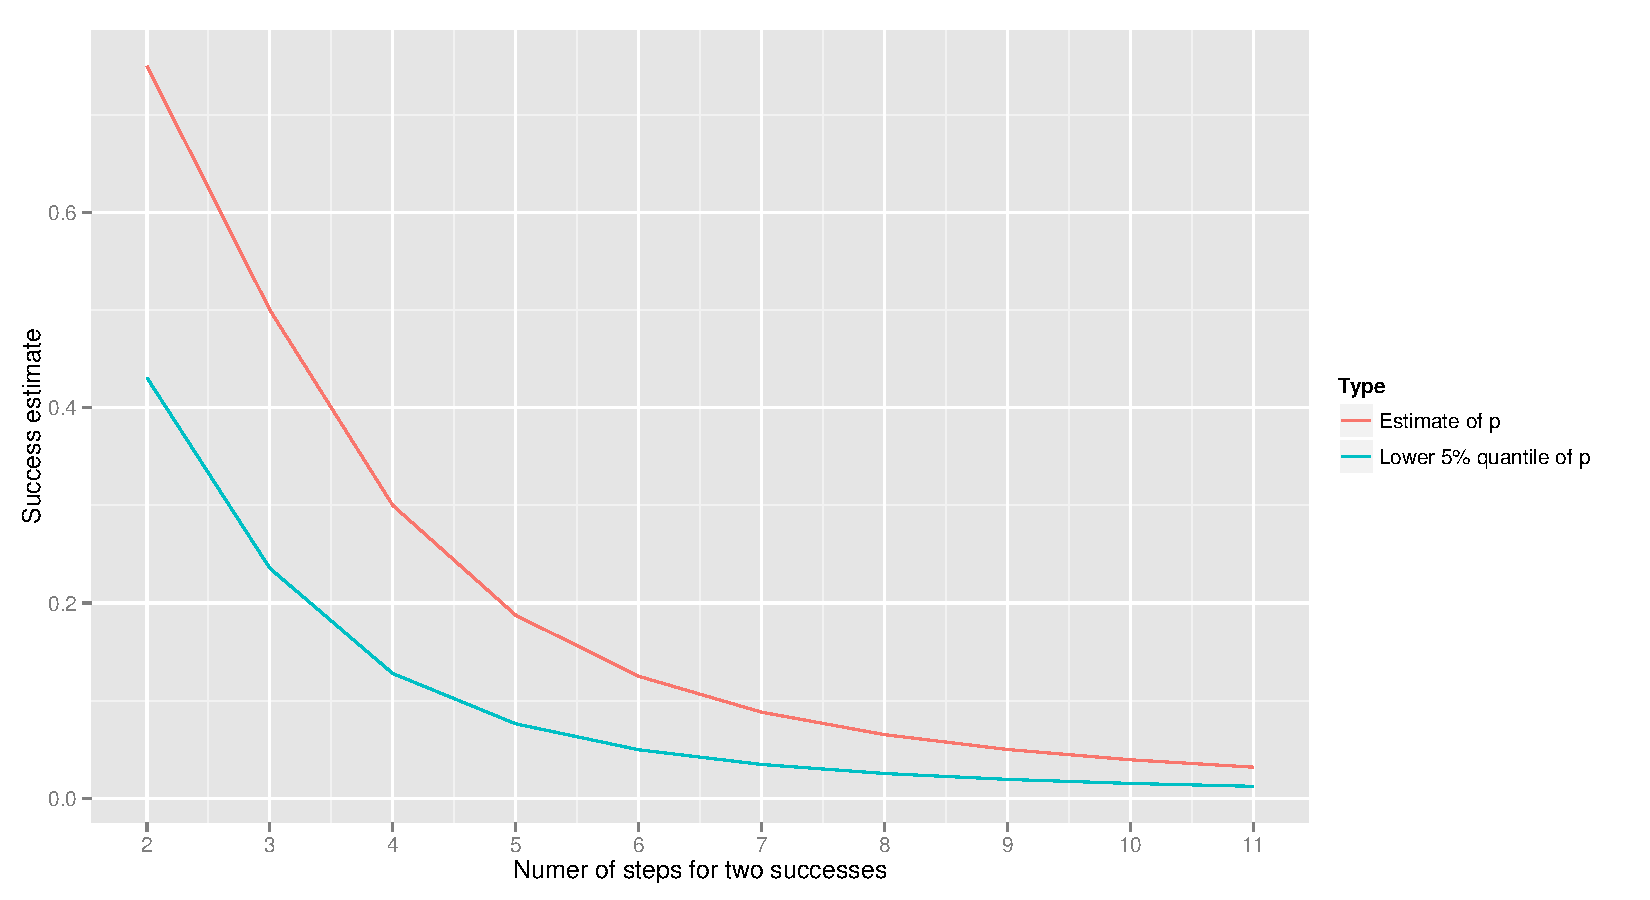
\includegraphics[width=\textwidth]{uncertainty.pdf}
\caption{
A visualization of the mode and the 0.05\% quantile of the estimate of the distribution of $p$.
}
\label{fig:simon}
\end{figure}

To better understand how the distributional estimate of $p$ changes in the number of steps needed for two successes data were simulated for each potential stopping point from two to 11. This procedure essentially estimates the shape parameters of a beta distribution. Fig. \ref{fig:simon} shows the change in the mode of the distribution, which is also the Maximum Likelihood Estimator (MLE) as well as the five percent quantile of the distribution. The graph shows, for example, that if a second success is found with the third enrollment then the MLE estimate of $p$ is 0.5 and with 95\% confidence $p$ is at least 0.25. In this case investigators could have moved on to the next stage of the trial with only three enrollments as opposed to 12.

\begin{table}
\begin{center}
\begin{tabular}{|c|c|c|} \hline
{\bf Steps to 2 successes} & {\bf Mode of $p$} & {\bf 5\% quantile} \\ \hline
2 & 0.7500  & 0.4307 \\ \hline
3 & 0.5000  & 0.2355 \\ \hline
4 & 0.3000  & 0.1278 \\ \hline
5 & 0.1875  & 0.0763 \\ \hline
6 & 0.1250  & 0.0497 \\ \hline
7 & 0.0882  & 0.0347 \\ \hline
8 & 0.0652  & 0.0254 \\ \hline
9 & 0.0500  & 0.0194 \\ \hline
10 & 0.0398 & 0.0153 \\ \hline
11 & 0.0319 & 0.0123 \\ \hline
\end{tabular} 
\end{center}
\caption{
A table of the mode and the 0.05\% quantile of the estimate of the distribution of $p$.
}
\label{tab:simon}
\end{table} 

Table \ref{tab:simon} shows the actual values used to generate Fig. \ref{fig:simon}. In the beginning of this section it was shown that, at the end of stage two, the breast cancer study actually tests whether the probability of success is greater than 0.0432 with 95\% confidence and requires 35 patients to do so. With the Stopped Negative Binomial model we only need six patients for the same level of confidence. This represents a tremendous amount of savings in time, effort and resources.

\subsection{Trial Monitoring}

Like most Bayesian Adaptive Clinical trials the SNB approach allows for monitoring of trial and can be updated as new results are received without losing power. Essentially this is because the object under investigation is not a point estimate of the success probability. It is the uncertainty in the distribution of the success probability. Point estimates of the success probability can be regarded as artifacts of our parameterization of the underlying distribution. Every point estimate calculated is accompanied by the quantification of the uncertainty around it. This estimate and it's uncertainty can be calculated at any time and may be useful in evaluating ongoing trials as well as providing a post-hoc evaluation of trials that have been completed.

\begin{figure}[ht]
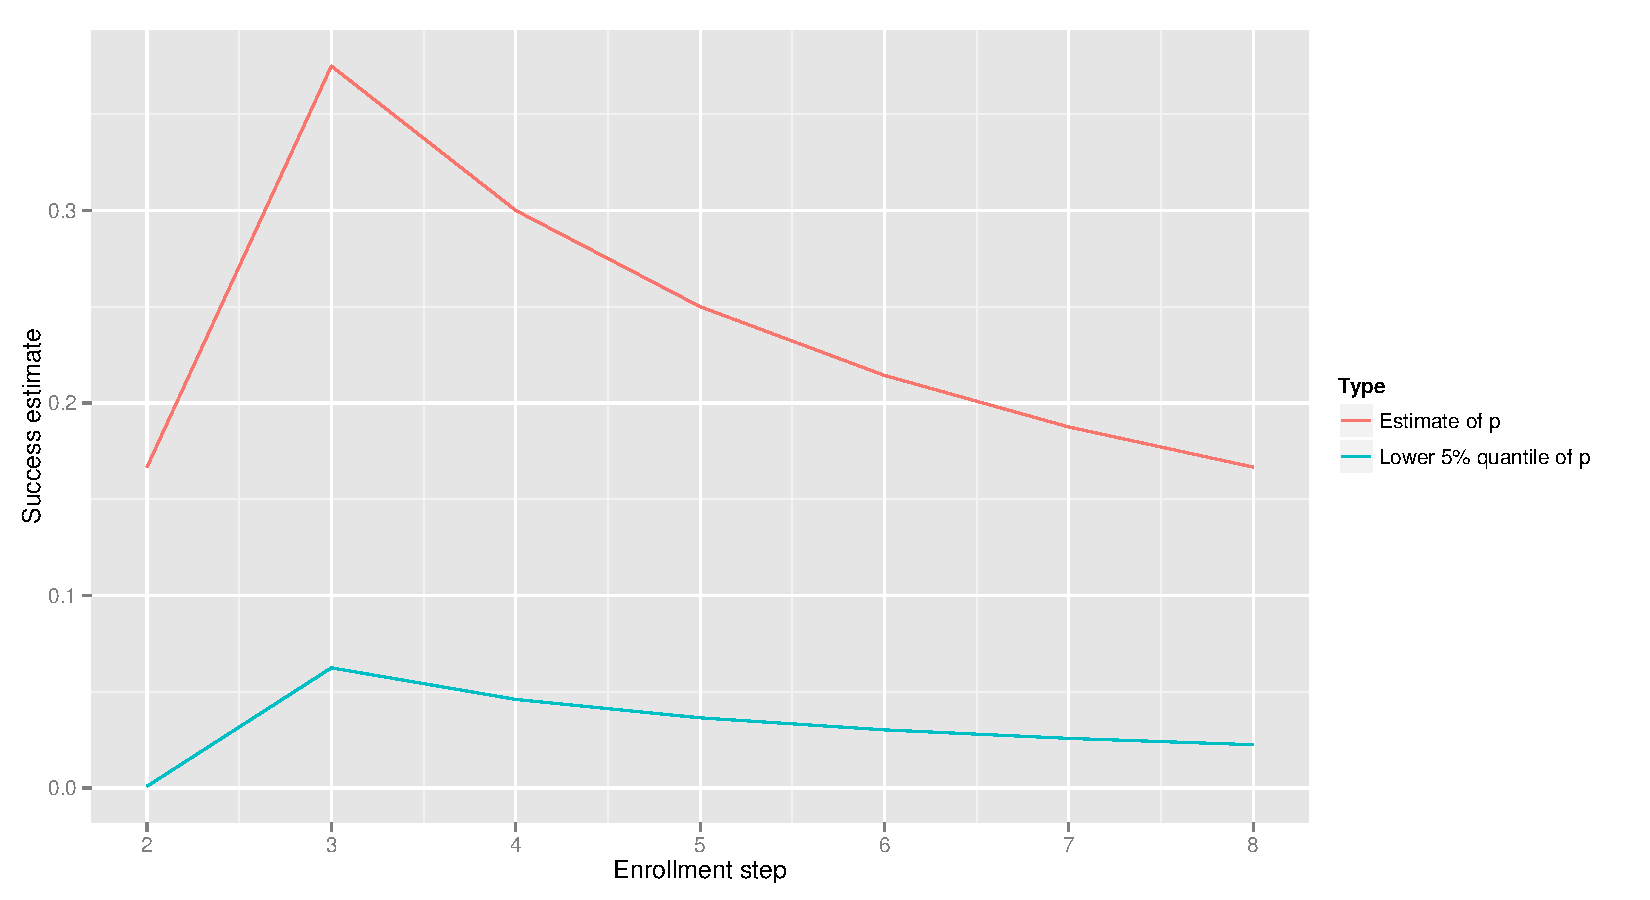
\includegraphics[width=\textwidth]{hypo_traj.pdf}
\caption{
A visualization of the mode and the 0.05\% quantile of the estimate of the distribution of $p$ for a hypothetical sequence of patient enrollments.
}
\label{fig:hypo}
\end{figure}

Consider the trial described above. Suppose eight patients were enrolled and there was a single success on the third trial (visualized in Fig. \ref{fig:hypo}). Since the mode of the beta distribution can only be calculated when there is at least one success the maximum of the mean and the mode of the distribution is shown as the estimate. At the third time step there is an increase in the estimate and the 0.05 \% quantile corresponding to the success. 

\begin{figure}[ht]
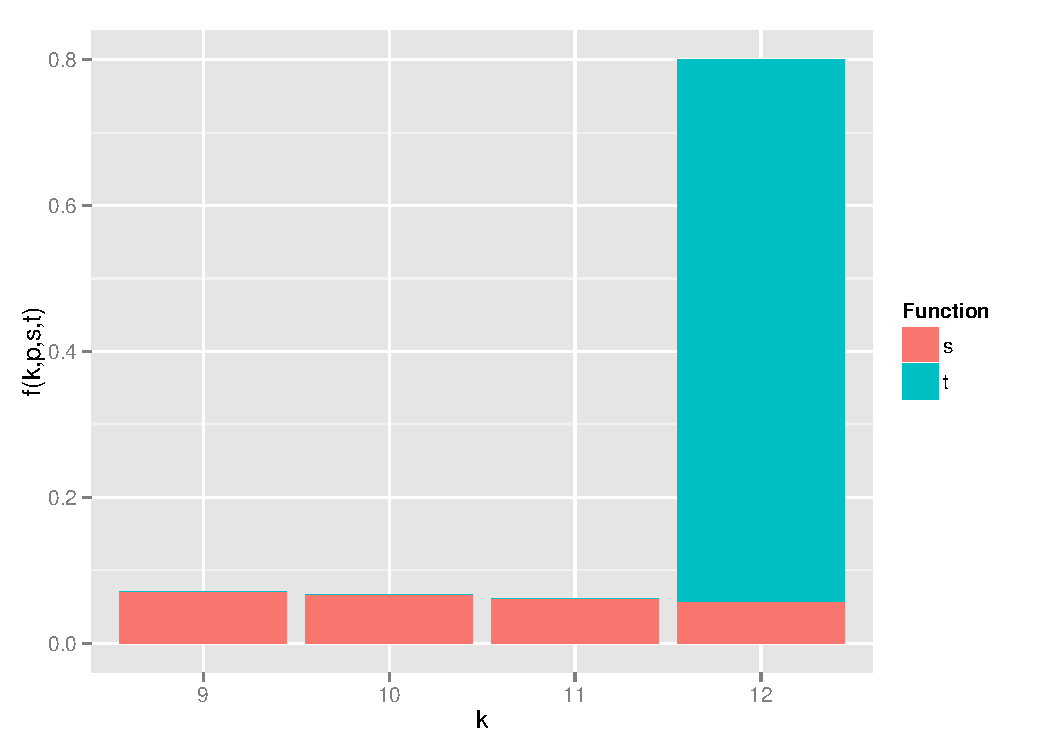
\includegraphics[width=\textwidth]{conditional_snb.pdf}
\caption{
The conditional Stopped Negative Binomial distribution after eight patients with one success.
}
\label{fig:conditional_snb}
\end{figure}

Fig. \ref{fig:conditional_snb} shows the conditional, compound SNB distribution. In each of the following enrollment a success would end the trial. If none of the following enrollments are success then the trial will stop at the eleventh patient. From Fig. \ref{fig:hypo} we know that the estimate of $p$ is about 0.19. The conditional compound distribution gives the probability of another success as 0.3883 and the probability of no more success (and the first stage failing) as 0.6117. Furthermore, we can see that the probability that the trial ends in the next step is approximately 20\% and the probability the trials end with the $11^{th}$ patient is about 65\%.

\subsection{Post-hoc Evaluation}

Suppose that in our example trial that a second successful outcome is reached on the $10^th$ patient. From the data collected we have shown how to create an estimate for the distribution of $p$. Based on that estimate we may like to see the probability of a different outcome. That is, what is the probability that we don't get two successful outcomes based on the data we have collected and what is the posterior distribution for the number of patients enrolled for the study?

In this case the success probability $p$ is distributed as $Beta(2.5, 8.8)$. Using the mode a point estimate yields $\hat{p} = 0.1667$. The standard deviation of the estimate is 0.1210. The probability of two successes during the trial is 0.6843 and the probability of failure is 0.3157. The distribution of the stopping times, along with contributions from two positive events and less than two positive events is shown below.

\begin{figure}[ht]
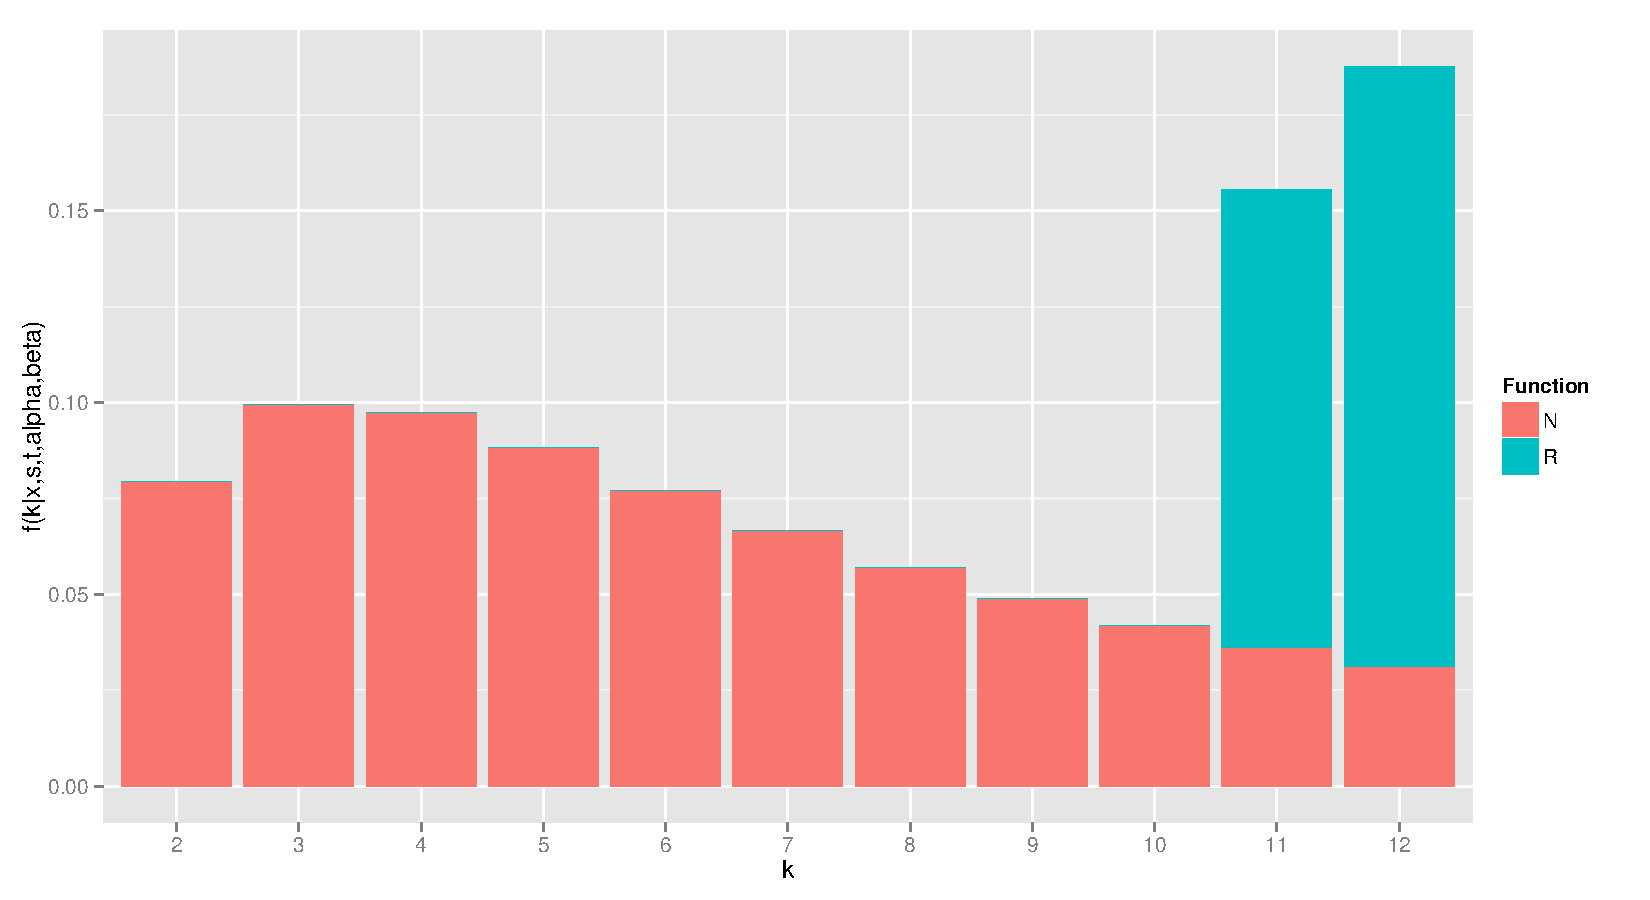
\includegraphics[width=\textwidth]{post_hoc.pdf}
\caption{
The post-hoc Stopped Negative Binomial distribution after the trial ends with 10 patient enrollments and two successes.
}
\label{fig:post_hoc}
\end{figure}

\section{Discussion and Conclusion}

We have presented a new discrete distribution by curtailed sampling rules common in early-stage clinical trials, which we refer to as the Stopped Negative Binomial distribution. The distribution models the stopping time of a sequential trial where the trial is stopped when a number of events are accumulated. The compound distribution was derived for the case when the event probability $p$ has a Beta distribution. Using a trial description from \url{clinicaltrials.gov} we showed how the SNB is an integral part of trial monitoring, and post-hoc analysis and can be used in a framework alternative to the Simon two-stage optimal design while providing better estimates of the event probability along with quantifying the uncertainty associated with the estimates. As a result, we were able to show fewer patient enrollments and achieve the same estimates, with added  in a hypothetical, but representative, clinical trial.

Current work focuses on the generalization of the distribution and the application in other areas of clinical trials. Adverse outcomes in particular are another area that could greatly benefit both from the presented distribution and its framework. For these trials monitoring may need to be performed not only on the outcome of an intervention but also on the safety of the trial. This especially in areas like late-stage cancer treatments where the treatment is harsh and patients may be forced to drop out as a result of the side-effects of the treatment; a matter independent of the outcome. Other application areas include providing design that allows clinicians to balance uncertainty and success probability with a minimum number of patient enrollees.

%   ------------------------    References     -----------------------


% -------------------------  References ---------------------------
\section*     {\bf References}
% -----------------------------------------------------------------


\begin{enumerate}

\item[\bibref{Kane 2015}]
Kane MJ. (2015). snb: The Stopped Negative Binomial. R package version 0.1. 2015. Available from \url{https://github.com/kaneplusplus/snb}

\item[\bibref{R Core Team 2015}]
R Core Team (2015). R: A language and environment for statistical
computing. R Foundation for Statistical Computing, Vienna, Austria. 2015. URL \url{http://www.R-project.org/}.

\item[\bibref{Sanofi 2013}]
Sanofi Pharmaceutical Company. A Phase 2, Single Arm Study of BSI-201 in Patients With BRCA-1 or BRCA-2 Associated Advanced Epithelial Ovarian, Fallopian Tube, or Primary Peritoneal Cancer. In: ClinicalTrials.gov [Internet]. Bethesda (MD): National Library of Medicine (US). 2000- [cited 2015 March 27]. Available from: \url{https://clinicaltrials.gov/ct2/show/study/NCT00677079} Identifier: NCT00677079.

\item[\bibref{Simon 1989}]
Simon R.  Optimal two-stage designs for Phase II clinical trials. {\it Controlled Clinical Trials\/} 1989; {\bf 10}: 1--10.

\item[\bibref{Uppuluri 1970}] 
Uppuluri VRR, Blot WJ. ``A probability distribution arising in a riff-shuffle.'' {\it Random Counts  in Scientific Work, 1: Random Counts in Models and Structures}, 1970. G.P. Patil (editor), University Park: Pennsylvania State University Press, pp  23--46.

\item[\bibref{Zhang 2000}]
Zhang Z, Burtness BA, Zelterman D.  The maximum negative binomial distribution. {\em Journal of Statistical Planning and Inference\/}  2000; {\bf 87}: 1--19.

\item[\bibref{Zelterman 2004}]
D Zelterman. {\it Discrete Distributions: Application in 
the Health Sciences}, New York: J. Wiley. 2004. xix + 277pp

\end{enumerate}

% ------------------------------------------------------------------




% ------------------------------------------------------------------
% --------------------   Tables and Figures   ----------------------
% ------------------------------------------------------------------




% -------------------------------------------------------------------


% -------------------------------------------------------------------
% ------------------------  FIGURES  --------------------------------
% -------------------------------------------------------------------

%\newpage 
% -------------------------------------------------------------------


%\newpage     %  Figure 1: functional forms of the mass function  


% -------------------------------------------------------------------

\end{document}

% ------------------  end of this file --------------------------



